\documentclass{article}
\usepackage{ctex}
\usepackage{amsmath}
\usepackage{geometry}
\usepackage{graphicx}
\usepackage{float} 
\usepackage{tikz}
\usetikzlibrary{positioning}
\usetikzlibrary{graphs,graphs.standard}
\tikzgraphsset{edges={draw,very thick}, nodes={circle,draw,thick}}
\usetikzlibrary{arrows.meta}
\graphicspath{{figure/}}
\geometry{a4paper,left=2cm,right=2cm,top=2cm}
\title{Discrete Mathematics Quiz 3\\\small{2021 - 2022 \enspace 春夏学期 \enspace 郑文庭班}}
\author{Shd0wash}
\date{\today}
\setlength{\parskip}{1em}
\setlength{\baselineskip}{20pt}
\setlength{\parindent}{0em}
\begin{document}

\maketitle

1. Find the transitive closure of $\mathit{R}$ on $\{a, b, c, d\}$, where $\mathit{R}$ = $\{(a, a), (b, a), (b, c), (c, a), (c, c), (c, d), (d, a), (d, c)\}$. (6\%)  

2.\\
(a) Find the smallest partial order relation $\mathit{R}$ on $\{a, b, c, d, e, f\}$ that contains $(a, c), (c, c), (c, b), (c, d), (b, e), (b, f)$.\\
(b) Draw the Hasse diagram of $\mathit{R}$.\\
(c) List the maximal elements.\\
(d) List the minimal elements.\\ 
(e) Find the greatest element.\\
(f) Find the least element.\\
(g) Find the least upper bound of $\{d, e\}$.\\
(h) Use topological sorting to order the elements of the poset. (24\%)  

3. Find a minimum spanning tree for the weighted graph in Fig.1. You can just draw out the answer. (6\%)  

\begin{figure}[htbp]
    \centering
    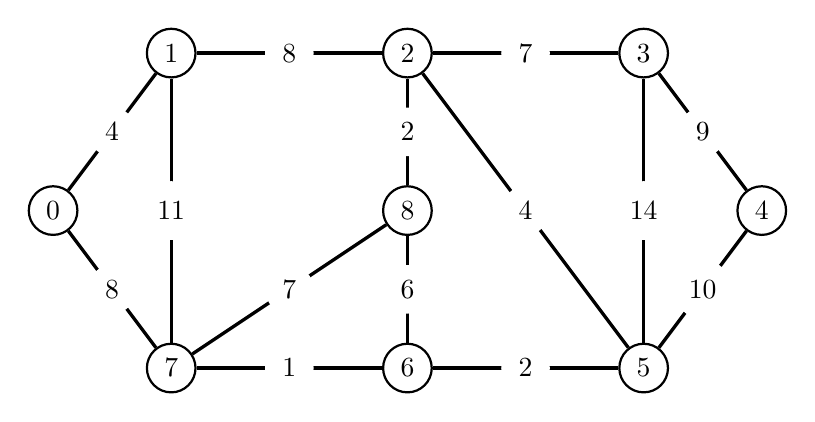
\begin{tikzpicture}
        \begin{scope}[every node/.style={circle,thick,draw}]
            \node (0) at (0,0) {0};
            \node (1) at (1.5,2) {1};
            \node (2) at (4.5,2) {2};
            \node (3) at (7.5,2) {3};
            \node (4) at (9,0) {4};
            \node (5) at (7.5,-2) {5};
            \node (6) at (4.5,-2) {6};
            \node (7) at (1.5,-2) {7};
            \node (8) at (4.5,0) {8};
        \end{scope}

        \begin{scope}[every node/.style={fill=white,circle},
            every edge/.style={draw=black,very thick}]
            \path [-] (0) edge node {$4$} (1);
            \path [-] (0) edge node {$8$} (7);
            \path [-] (1) edge node {$8$} (2);
            \path [-] (1) edge node {$11$} (7);
            \path [-] (2) edge node {$7$} (3);
            \path [-] (2) edge node {$4$} (5);
            \path [-] (2) edge node {$2$} (8);
            \path [-] (3) edge node {$9$} (4);
            \path [-] (3) edge node {$14$} (5);
            \path [-] (4) edge node {$10$} (5);
            \path [-] (5) edge node {$2$} (6);
            \path [-] (6) edge node {$1$} (7);
            \path [-] (6) edge node {$6$} (8);
            \path [-] (7) edge node {$7$} (8);
        \end{scope}
    \end{tikzpicture}
    \caption{Fig.1}
\end{figure}

\clearpage

4. Use Dijkstra's Algorithm to find the shortest path length between the vertices 1 and 6 in the weighted graph in Fig.2. (10\%)

\begin{figure}[htbp]
    \centering
    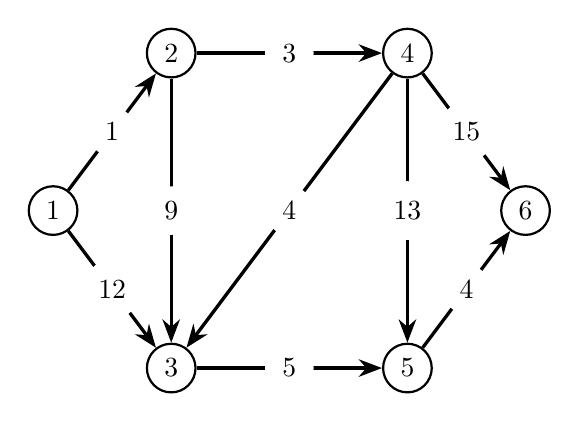
\begin{tikzpicture}
        \begin{scope}[every node/.style={circle,thick,draw}]
            \node (1) at (0,0) {1};
            \node (2) at (1.5,2) {2};
            \node (3) at (1.5,-2) {3};
            \node (4) at (4.5,2) {4};
            \node (5) at (4.5,-2) {5};
            \node (6) at (6,0) {6};
        \end{scope}

        \begin{scope}[>={Stealth[black]},
            every node/.style={fill=white,circle},
            every edge/.style={draw=black,very thick}]
            \path [->] (1) edge node {$1$} (2);
            \path [->] (1) edge node {$12$} (3);
            \path [->] (2) edge node {$9$} (3);
            \path [->] (2) edge node {$3$} (4);
            \path [->] (3) edge node {$5$} (5);
            \path [->] (4) edge node {$4$} (3);
            \path [->] (4) edge node {$13$} (5);
            \path [->] (4) edge node {$15$} (6);
            \path [->] (5) edge node {$4$} (6);
        \end{scope}
    \end{tikzpicture}
    \caption{Fig.2}
\end{figure}

5. Use Huffman coding to encode these symbols with given frequencies: a: 0.15, b: 0.22, c: 0.26, d: 0.19, e: 0.08, f: 0.1. What is the average number of bits required to encode a character? (8\%)

6. Determine all positive integers $\mathit{r}$ and $\mathit{s}$ for which $\mathrm{K}_{r,s}$ is planar. Explain your answer. (8\%)

7. In a round-robin tournament every player plays every other player exactly once and each match has a winner and a loser. There are total $\mathit{n}$ players. Prove that we can sort the players in a certain order 
$p_{1}, \enspace p_{2}, \enspace \ldots , \enspace p_{n}$, so that $p_{1}$ beats $p_{2}$, $p_{2}$ beats $p_{3}$, $\ldots$, and $p_{n-1}$ beats $p_{n}$. (10\%) 

8. Fig.3 is the Petersen graph. (28\%)\\
(a) Find the chromatic number of the Petersen graph.\\
(b) Determine whether the graph in Fig.4 is also a Petersen graph.\\
(c) Prove that the Petersen Graph is non-planar using Euler's formula.\\
(d) Determine whether the Petersen graph is Hamilton graph. Prove or disprove it.
\begin{figure}[htbp]
    \centering
    \begin{minipage}[t]{0.48\textwidth}
        \centering
        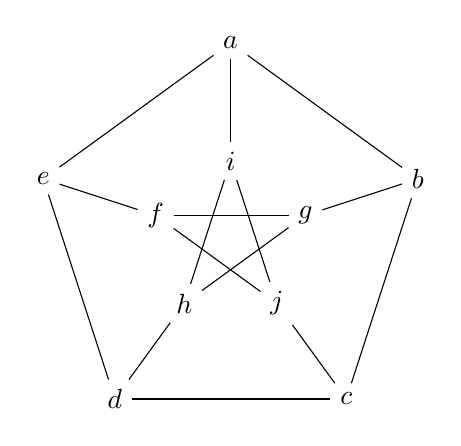
\begin{tikzpicture}
            \graph[math nodes, clockwise]{ 
                subgraph I_n [V={i,g,j,h,f}] --
                subgraph C_n [V={a,b,c,d,e},radius=1.5cm];
                {[cycle] f,g,h,i,j} };
        \end{tikzpicture}
        \caption{Fig.3}
    \end{minipage}
    \begin{minipage}[t]{0.48\textwidth}
        \centering
        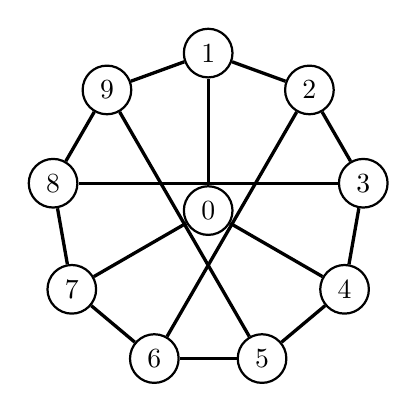
\begin{tikzpicture}
            \begin{scope}[every node/.style={circle,thick,draw}]
                \node (0) at (0,0) {0};
                \node (1) at (90:2) {1};
                \node (2) at (50:2) {2};
                \node (3) at (10:2) {3};
                \node (4) at (-30:2) {4};
                \node (5) at (-70:2) {5};
                \node (6) at (-110:2) {6};
                \node (7) at (-150:2) {7};
                \node (8) at (170:2) {8};
                \node (9) at (130:2) {9};
            \end{scope};

            \begin{scope}[every node/.style={fill=white,circle},
                every edge/.style={draw=black,very thick}]
                \path [-] (1) edge (2);
                \path [-] (2) edge (3);
                \path [-] (3) edge (4);
                \path [-] (4) edge (5);
                \path [-] (5) edge (6);
                \path [-] (6) edge (7);
                \path [-] (7) edge (8);
                \path [-] (8) edge (9);
                \path [-] (9) edge (1);
                \path [-] (0) edge (1);
                \path [-] (0) edge (4);
                \path [-] (0) edge (7);
                \path [-] (3) edge (8);
                \path [-] (2) edge (6);
                \path [-] (9) edge (5);
            \end{scope}
        \end{tikzpicture}
        \caption{Fig.4}
    \end{minipage}
\end{figure}
\end{document}